\documentclass{report}
\usepackage{polski}
\usepackage[utf8]{inputenc}
\usepackage[margin=1in,left=1.5in,includefoot]{geometry}
\usepackage{fancyhdr}
\pagestyle{fancy}

\usepackage{graphicx}
\graphicspath{ {./images/} }

\begin{document}

\begin{titlepage}

\title{Praca inżynierska}
\author{Kamil Susek}
\date{September 2020}

\maketitle
\end{titlepage}
\chapter{Wprowadzenie}
\newpage
\chapter{Blockchain}
Technologia Blockchain to stosunkowo nowe rozwiązanie. Pierwsze zastwosowanie tej technologii miało miejsce w roku 2009, w popularnej kryptowalucie bitcoin. Zadaniem Blockchainu było księgowanie transakcji. Od tego czasu można zauważyć zwiększanie się zainteresowania tą technologią, co przekłada się na powstawanie nowych kryptowalut i nowych rozwiązań Blockchain (Blockachain 2.0, 3.0).
\section{Architektura Blockchain}
Blockchain to łańcuch bloków, które przechowują dane. Każdy blok przechowuje zabezpieczone kryptograficznie informacje, o poprzednim bloku i w ten sposób tworzy się trudny do modyfikacji łańcuch. Technologia blockchain wykorzystuje rozproszoną sieć, w celu przechowywaniu kopii łańcucha w zdecentralizowanym systemie. Takie rozwiązanie pozwala zwiększyć bezpieczeństwo przechowywanych danych.
\subsection{Łańcuch bloków}
Łańcuch bloków w systemie Blockchain pełni funkcje struktury danych. Jego budowa przypomina trochę listę jednokierunkową, jednak zamiast wskaźników na poprzedni element, blok przechowuje hash poprzedniego elementu. Hash to wygenerowany za pomocą odpowiedniej funkcji kryptograficznej (funkcji skrótu) ciąg bajtów. Hashowanie jest operacją jednokierunkową, co oznacza brak możliwości odczytania danych wejściowych na podstawie wartości wygenerowanej przez hash.
Do popularnych funkcji skrótu należą SHA i MD5, jednakże należy pamiętać, że co jakiś czas te rozwiązania się zmieniają, ponieważ odkrywane są w nich luki.

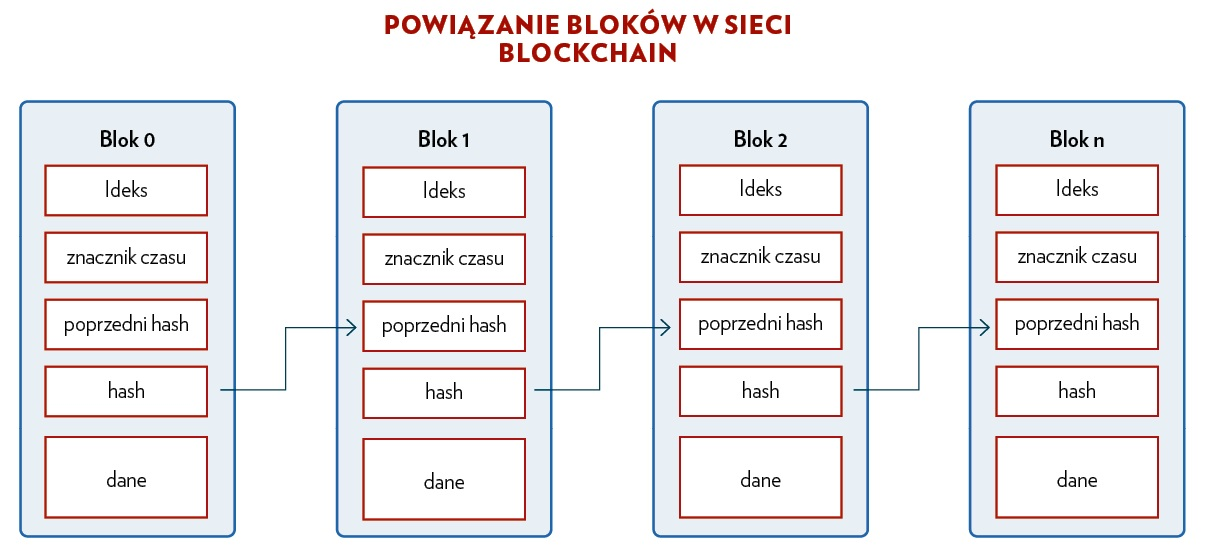
\includegraphics[width=\textwidth]{images/łańcuch_bloków.jpg}

Na łańcuchu bloków, jak na każdej strukturze danych można wykonywać jakieś operacje. W tym przypadku jednak operacje takie jak usuwanie bloku, lub jego modyfikacja nie mają sensu, ponieważ mechanizmy zastosowane w łańcuchu mają na celu zabezpieczenie przed modyfikacją danych w bloku. Najczęściej wykorzystuje się operacje dodawania bloku i sprawdzenia spójności łańcucha.

Dodanie bloku to dołączenie do tablicy bloków (bądź innej struktury łączącej lub indeksującej bloki) nowego bloku, w którym w pole "poprzedni hash" wpisywana jest wartość hash poprzedniego bloku. Następnie w świeżo dodanym bloku z wykorzystaniem funkcji skrótu liczymy hash z pól przechowujących dane, poprzedni hash i znacznik czasu.  

Sprawdzenie spójności łańcucha to przeliczenie hasha każdego bloku i porównanie go z polem "poprzedni hash" następnego bloku. Jest to główny mechanizm pozwalający wykryć niespójność w łańcuchu bloków, lecz nie należy tego mylić z problemem niespójności, w rozproszonym systemie Blockchain.


\newpage
\chapter{Analiza dziedziny}
Elektroniczne systemy głosowania coraz bardziej zyskują na popularności.
Wraz z postępem technologii oraz coraz większego znaczenia internetu w życiu 
społecznym, pojawiają się pomysły (a nawet implementacje) przeniesienia procesu głosowania do sieci. Pomysły i implementacje internetowych systemów wyborczych dotyczą wyborów na szczeblu państwowym (przykładowo wybory prezydenckie), jak i wyborów organizowanych na potrzeby prywatne. System e-votingu zazwyczaj sprowadza się do serwisu internetowego, który pozwala na oddanie głosu poprzez odpowiednią stronę internetową. 

Przeniesienie głosowania do aplikacji internetowej, pozwala zminimalizować wpływ ewentualnego błędu ludzkiego podczas przeprowadzania wyborów. Jednakże takie rozwiązanie generuje nowe problemy, z którymi muszą się zmierzyć projektanci tych systemów. Największy problem stanowi zabezpieczenie aplikacji, przed zewnętrznymi próbami fałszowania wyników głosowania. Rozwój technologii prowadzi również do powstawania nowych odmian “złośliwego oprogramowania”, co prowadzi do ciągłego aktualizowania zabezpieczeń. Aplikacja odpowiadająca na potrzeby wyborów, na wysokim szczeblu powinna być tworzona “na potrzeby danych czasów”, bądź łatwa w płynnej aktualizacji.

Zabezpieczenie przed fałszowaniem głosów to nie jest jedyny problem, z jakim trzeba się zmierzyć podczas próby przeniesienia procesu głosowania do internetu. Kolejnym problemem jest sama logika systemu głosowania, niektóre wybory wymagają, aby informacje o wyborcach oraz ich głosach, były tajne. System powinien również umożliwiać weryfikację użytkownika, na podstawie dostarczonych przez organizatora wyborów danych logowania. Coraz głębsza analiza problemu generuje coraz więcej potrzeb z zakresu bezpieczeństwa systemu. Dodatkowo wyszczególniając elementy, które powinny podlegać szczególnej protekcji należy zadbać, aby architektura systemu pozwalała na łatwą aktualizację zabezpieczeń.

Wykorzystując komputery do obsługi głosowania, oczekuje się szybkiego i poprawnego uzyskania rezultatu głosowania. System taki powinien być zoptymalizowany, a czas uzyskania rezultatów powinien być deterministyczny. Warto rozważyć także moduł generujący statystyki wyborcze.

System wyborczy to nie tylko serwer, który zbiera, przechowuje i liczy głosy. Kliencka część aplikacji (widoczna dla wyborcy) powinna być responsywna, przejrzysta oraz przyjazna dla osób z pewnymi niepełnosprawnościami (głównie należy uwzględnić wady wzroku).

Dużą zaletą e-votingu jest przeniesienie procedur, które musi wykonać organizator do interaktywnej aplikacji przeglądarkowej. Aplikacja webowa powinna zapewniać możliwość zarządzania głosowaniem oraz kreator głosowania, ten element również powinien podlegać zabezpieczeniu danych i autentykacji użytkownika. Aplikacja wyposażona w takie funkcjonalności powinna spełniać wymagania elektronicznego systemu głosowania.

\section{Wstępne wymagania niefunkcjonalne}
Z powyższej analizy można wypunktować następujące wymagania:
\begin{itemize}

\item Dbałość o zabezpieczenie głosu wyborcy przed fałszerstwem - rezultat głosu nie może zostać zmieniony, po jego zatwierdzeniu.

\item Zabezpieczenie danych wyborcy, poprzez utajnienie jego tożsamości.

\item Sprawne i bezbłędne liczenie głosów - czas liczenia głosów powinien być deterministyczny.

\item Dbałość o prezencję aplikacji, strona kliencka powinna być przejrzysta i łatwa w obsłudze.

\item System musi być konfigurowalny, z uwzględnieniem bezpieczeństwa konfiguracji.
\end{itemize}


\section{Przegląd istniejących rozwiązań e-votingu}
Dokonana analiza jest wstępną analizą, która nie jest wystarczająco szczegółowa. Idealna aplikacja, jest dopracowana w najmniejszych detalach. W celu doprecyzowania wymagań można dokonać przeglądu i analizy istniejących rozwiązań. Analizując istniejące aplikacje można wyciągnąć wiele przydatnych wniosków.
\section{System estoński}
Przykładem regularnego wykorzystania e-votingu jest Estonia. Estonia jest krajem, który pierwszy udostępnił możliwość głosowania elektronicznego w wyborach lokalnych, na szczeblu krajowym. W pierwszych wyborach wzięło udział około 1\% wyborców. Od roku 2005 w Estonii postępował rozwój systemów e-votingu. Wraz z następnymi wyborami zwiększała się liczba uczestników. W roku 2019 liczba wyborców, którzy skorzystali z e-votingu wyniosła 43,8\% wyborców.

Na system e-votingu  w Estonii składa się kilka mniejszych rozwiązań, które można wylistować w następujący sposób:
\begin{itemize}

    \item Identyfikacja za pomocą karty e-obywatela lub profilu e-obywatela w telefonie.

    \item Architektura rozwiązania pozwala na wysłanie wielu głosów, a głosem wiążącym jest zawsze głos finalny.

    \item Serwery wykorzystywane podczas głosowania są pod szczególną ochroną i nie można uzyskać do nich dostępu z bezpośrednio z internetu (zabezpieczenie firewallem).

    \item Wykorzystywanie prywatnych kluczy i narzędzi kryptograficznych w celu zabezpieczenia dostępu do danych. Wykorzystywanie standardu SSL.
    
\end{itemize}

\subsection{Przegląd rozwiązania}
Przebieg całego procesu wyborczego w Estonii można podzielić na kilka etapów:
\begin{itemize}
    \item ogłoszenie wyborów;
    \item zarejestrowanie kandydat;
    \item przygotowanie list wyborczych;
    \item głosowanie;
    \item liczenie głosów;
    \item ogłoszenie wyników;
\end{itemize}

Wsparcie e-votingu (w Estonii określanego i-votingiem) obejmuje ostatnie trzy etapy procesu wyborczego.

\includegraphics[width=\textwidth]{images/Dziedzina systemu estońskiego}

W skład systemu głosowania wchodzą bazy danych przechowujące:
\begin{itemize}
    \item listę osób uprawnionych do głosowania;
    \item listę okręgów wyborczych;
    \item listę kandydatów lub opcji wyborczych;
    \item listę e-wyborców (i-voters);
\end{itemize}

Dostarczenie odpowiednich danych do systemu pozwala na walidację wyborcy, zgłoszenie przez 
niego głosu oraz zapisanie wyborcy, w bazie danych odpowiedzialnej za przechowanie listy e-wyborców. W skład logiki systemu wchodzą mechanizmy generujące wyniki. Wyniki e-votingu są scalane z wynikami wyborów tradycyjnych, przy czym scalanie nie pozwala na podwójne zliczenie głosu oddanego tradycyjnie i elektronicznie.


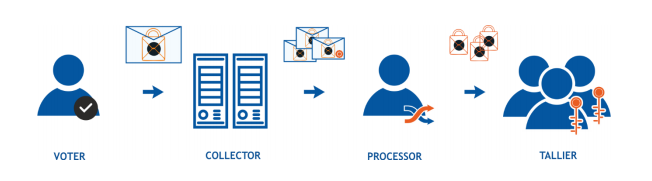
\includegraphics[width=\textwidth]{images/Główne częsci systemu estońskiego.png}

Główne częsci systemu:
\begin{itemize}
    \item Voter (dalej nazywany wyborcą) - za pośrednictwem aplikacji klienckiej (która w systemie estońskim jest aplikacją desktopową pobieraną przed wyborami) szyfruje i zatwierdza swoim podpisem elektronicznym głos, który następnie wysyłany jest do Kolektora.
    \item Collector (dalej nazywany Kolektorem) - to aplikacja serwerowa wyposażona w logikę pozwalającą na utworzenie głosu. Aplikacja waliduje dane wprowadzone przez wyborce i elektronicznie podpisuje dane, które następnie przesyła do Procesora.
    \item Processor (dalej nazywany Procesorem) - zajmuje się przetwarzaniem głosów. Sprawdza poprawność danych otrzymanych z Kolektora, wraz z podpisem elektronicznym. Usuwa głosy, które się powtarzają, zarówno głosy oddane elektronicznie, jak i te oddane w lokalach wyborczych. Sortuje głosy według okręgów wyborczych i usuwa z nich podpis elektroniczny, w celu anonimizacji głosu. Tak przetworzone głosy są mieszane według odpowiedniego algorytmu i wysyłane do Licznika.
    \item Tallier (dalej nazywany Licznikiem) - rolą licznika jest odebranie głosu od Procesora, otwarcie go i dodanie przyporządkowanie do odpowiedniego wyniku.
\end{itemize}
\chapter{Projekt systemu}
\section{Moduły systemu}
Całość aplikacji dzieli na moduły, które komunikując się ze sobą tworzą działający system. Taki podział pozwala na zwiększenie przejrzystości architektury aplikacji i ułatwienie jej testowania.
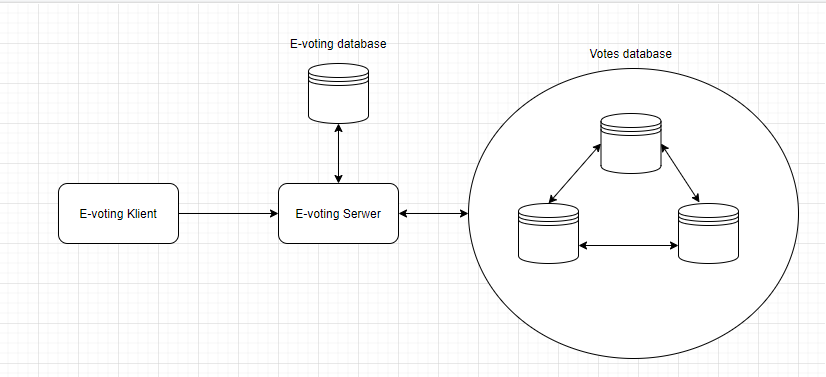
\includegraphics[width=\textwidth]{images/podział_na_moduły.png}
Aplikacja jest podzielona na stronę serwerową i kliencką. Jest to rodzaj architektury systemów oprogramowania nazywany "klient-serwer". Aplikacje typu "klient-serwer" są bardzo popularne w środowisku aplikacji webowych, które wykorzystują bazę danych. Głównym założeniem takiego podejścia jest przeniesienie do aplikacji klienckiej, tego co widzi użytkownik (UI, UX, interakcje z użytkownikiem) i wyodrębnienie logiki aplikacji, zapytań do bazy danych oraz przetwarzania danych do aplikacji serwerowej. Aplikacja serwerowa odpowiada na żądania klienta. Działanie takiego systemu odbywa się przez odpowiedni protokół komunikacyjny (np. UDP, TCP).



W przypadku projektowanego systemu strona serwerowa jest podłączona do dwóch baz danych. E-voting database dostarcza dane związane z wyborcami i wyborami, baza jest zorganizowana w modelu obiektowo-relacyjnym (ORM).

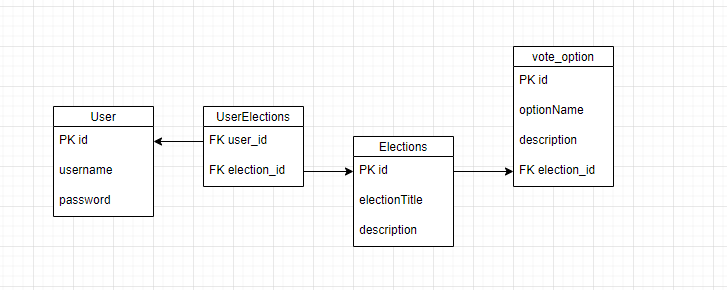
\includegraphics[width=\textwidth]{images/Baza_danych.png}

Natomiast daza danych "Votes database" to sieć rozproszonych baz danych przechowująca wpisy z oddanymi głosami. Struktura tej bazy danych to tzw. Blockchain. Każdy węzeł tej sieci przechowuje łańcuch bloków, gdzie każdy blok zawiera transakcje z oddanym głosem. Każdy węzeł powinien posiadać taką samą zawartość łańcucha bloków, w przeciwnym razie należy zweryfikować i zaktualizować zawartość łańcucha bloków.

\end{document}
